\documentclass[tikz,border=10pt]{standalone}
\begin{document}
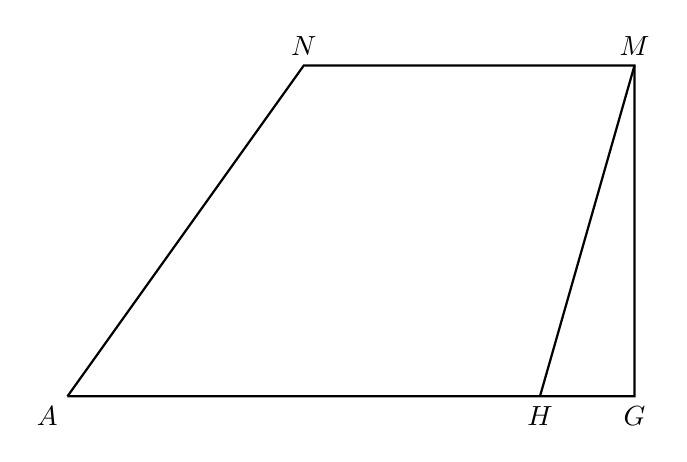
\begin{tikzpicture}[scale=1.2]
\coordinate (A) at (0,0);
\coordinate (H) at (5,0);
\coordinate (G) at (6,0);
\coordinate (N) at (2.5,3.5);
\coordinate (M) at (6,3.5);

\draw[thick] (A) -- (N) -- (M) -- (G) -- (A);
\draw[thick] (M) -- (H);

\node[below left] at (A) {$A$};
\node[below] at (H) {$H$};
\node[below] at (G) {$G$};
\node[above] at (N) {$N$};
\node[above] at (M) {$M$};
\end{tikzpicture}
\end{document}
